\section{Transmisión de datos en banda ancha}
La banda ancha surge de la necesidad de cambiar la utilidad de las redes clásicas, es decir, adaptarse a las nuevas necesidades. Ahora las redes se usan más para la transmisión de datos que de voz.\\
Las redes se dividirán en:
\begin{itemize}
\item Red de acceso, conecta al usuario con la red.
\item Red troncal, secciones internas de las grandes redes de los proveedores de internet(ISP).
\end{itemize}
Al principio se optó por opciones como la Jerarquía Digital Plexincrona (PDH). Los sistemas MIC agrupan canales de 64kbps. El sistema MIC de norma europea agrupa 30 canales produciendo 2Mbps de transmisión y el americano 24 canales produciendo 1.5Mbps de transmisión.
\subsection{RDSI}
La Red Digital de Servicios Integrados(RDSI) es la siguiente evolución y ofrece dos canales por terminalque se podrán utilizar de la forma que cada uno decida. Este sistema tiene un latencia muy baja que aún no se ha podido igualar. Se utiliza TDM con un envío de un paquete de 8 bits cada 125 microsegundos.
\subsubsection{Estructura RDSI}
Como se puede ver en la imagen la estructura del RDSI es muy simple. La sección del ISP termina en TR1 que es la roseta de entrada a casa.
\begin{figure}[htp]
	\centering
	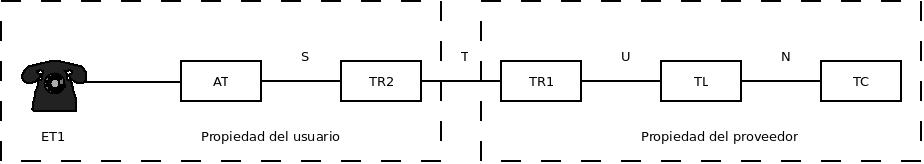
\includegraphics[width=\textwidth]{Imagen/diaRDSI.jpg}
	\caption{Estructura del sistema RDSI}
	\label{}
\end{figure}
Las difierentes piezas de la estructura son:
\begin{itemize}
	\item ET1: estación terminal. Con acceso básico podrían colocarse 2 terminales. estos son ordenadores, telefonos, etc.
	\item AT: este módulo se utiliza para adaptar telefonos analógicos al sistema digital. Este no siempre es necesario.
	\item TR2: una centralita de distribución, separa los canales para los diferentes terminales. No siempre hay uno
	\item TR1: roseta de entrada. Primer elemento perteneciente al ISP.
	\item TL y TC: son parte de la central local.
\end{itemize}
Las interfaces que conectan los anteriores son:
\begin{itemize}
	\item Interfaz S: 192kbps
	\item Interfaz T
	\item Interfaz U: 160kbps en acceso básico y 2mbps (europa), 1.5mbps (américa) en acceso primario.
	\item Interfaz N
\end{itemize}
Las interfaces S y T presentan la peculiaridad de ser iguales electricamente, es decir en caso de que no halla un TR2 la estación terminal se puede conctar directamente a la roseta. Esto no quita que en caso necesario las modulaciones o accesos multiples se puedan diferenciar.\\
\subsubsection{Accesos}
Los diferentes accesos se configuran en función de la configuración de diferentes canales.
\begin{itemize}
	\item Canal B: Transmite infromación a una velocidad de 64kbps.
	\item Canal D: Es un canal de señalización que va entre 16 y 64 kbps.
	\item Canal H: Transmite información a una velocidad superior a 64kbps.
\end{itemize}
Un acceso básico incluye dos canales B y un canal D (a 16kbps). Un acceso primario coincide con los sistemas MIC del sistema PDH. El acceso primario se constituye de 30 canales B y un canal D (a 64kbps) en europa y 23 canales B en américa.
\subsection{Banda ancha en núcleo de abonado xDSL}
Utilización del bucle de abonado más allá del telefono. Hace uso de modulaciones multiportadora adaptada. Se analiza el canal y se diseña en que frecuencias se utilizan que modulaciones para utilizar mejor el ancho de banda. En algunos casos por la cercania entre bandas es necesaria la utilización de cancelación de ecos.
\subsection{SDH}
Conjunto jerárquico de estructuras digitales de transporte de cargas adaptadas sobre redes de transmisión física". Se trata de una técnica de multiplexación utilizada normalmente en los sistemas de fibra óptica. Ha sido adaptado también a sistemas de cable coaxial.\\
El SDH utiliza como unidad básica el STM-1 (Módulo de Transferencia Sincrona). en la figura se puede ver la estructura lógica de un STM-1.
\begin{figure}[H]
\centering
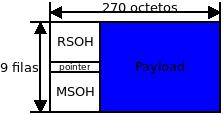
\includegraphics[width=0.7\textwidth]{Imagen/diaSTM1.jpg}
\caption{Estructura lógica de la trama STM-1}
\label{}
\end{figure}
\begin{itemize}
	\item Payload: Donde se guardan los datos enviados por los usuarios.
	\item RSOH: Cabezera de regeneración (al ser fibra hey que regenerar la señal cada poco espacio. CRC's, etc.
	\item MSOH: Cabezera de multiplexación, número de cargas, posición de cada una de ellas, etc.
	\item Pointer: Puntero al inicio de la carga util.
\end{itemize}
En la siguiente figura se puede ver la estructura seguida para la multiplexación de los diferentes contenedores de carga.
\begin{figure}[H]
\centering
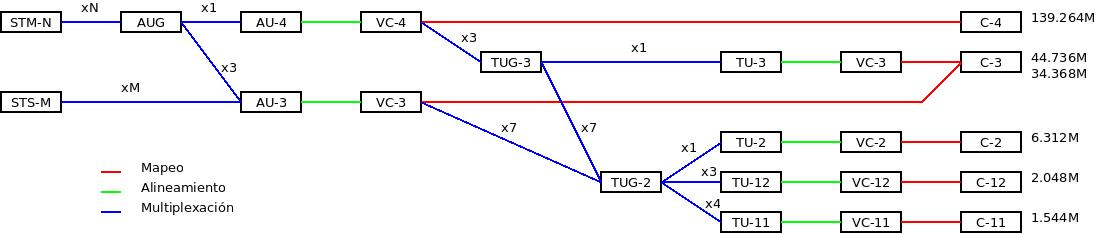
\includegraphics[width=\textwidth]{Imagen/diamuxSDH.jpg}
\caption{Estructura de la multiplexación en SDH}
\label{}
\end{figure}